\documentclass{standalone}
% main document, called main.tex

% \usepackage{newtxtext}       %
% \usepackage{newtxmath}   
\usepackage{amsmath}   
\usepackage{amssymb}   

\newcommand\szcirc{0.36cm}

\usepackage{tikz}

\begin{document}

\newcommand{\juv}{S}

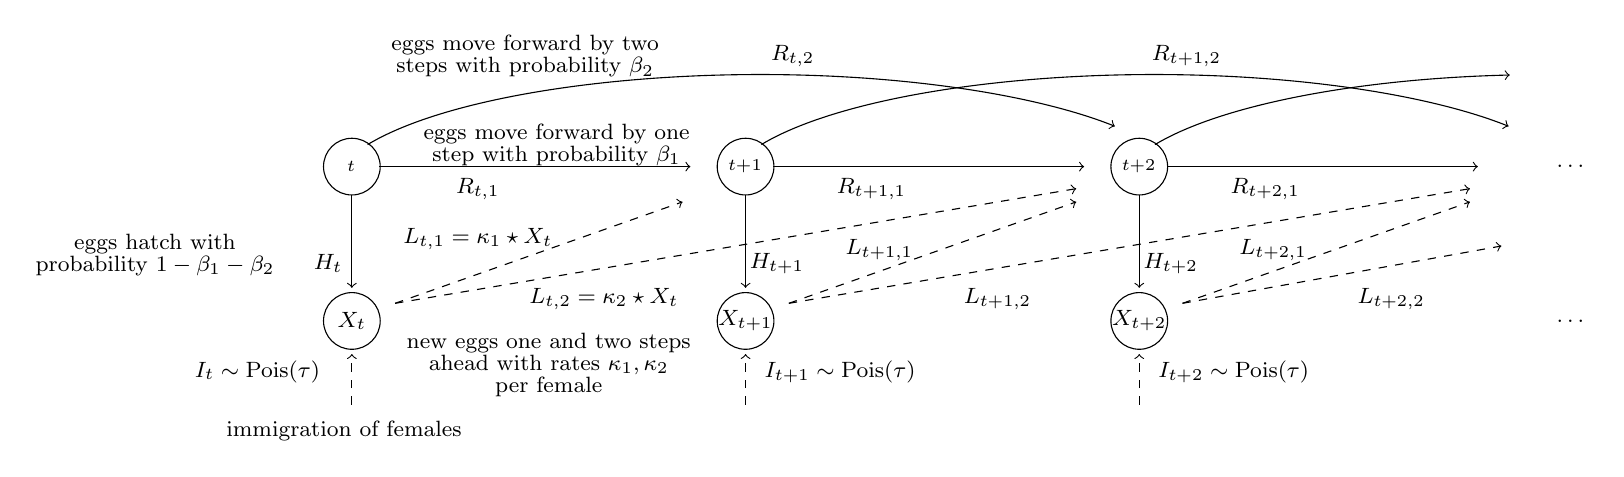
\begin{tikzpicture}[x=1cm,y=0.28cm]
\footnotesize
% two place holders to get some margins:
% \draw[white,fill=white](6,1) node {};
% \draw[white,fill=white](6,1) node {};

% circles:
\draw[black,fill=white](11,3) circle (\szcirc) node {$\juv_{t}$};
% \draw[black,fill=white](11,-3) circle (\szcirc) node {$H_{t}$};

\draw[black,fill=white](11,-4) circle (\szcirc) node {$X_{t}$};
% \draw[black,fill=white](11,-11) circle (\szcirc) node {$I_{t}$};

\draw[black,fill=white](16,3) circle (\szcirc) node {$\juv_{t + 1}$};
% \draw[black,fill=white](16,-3) circle (\szcirc) node {$H_{t + 1}$};
\draw[black,fill=white](16,-4) circle (\szcirc) node {$X_{t + 1}$};
% \draw[black,fill=white](16,-11) circle (\szcirc) node {$I_{t + 1}$};

\draw[black,fill=white](21,3) circle (\szcirc) node {$\juv_{t + 2}$};
% \draw[black,fill=white](16,-3) circle (\szcirc) node {$H_{t + 1}$};
\draw[black,fill=white](21,-4) circle (\szcirc) node {$X_{t + 2}$};
% \draw[black,fill=white](16,-11) circle (\szcirc) node {$I_{t + 1}$};

% dots right
\draw[black,fill=white](26.5,3) node {$\dots$};
\draw[black,fill=white](26.5,-4) node {$\dots$};

% long horizontal arrows:
\foreach \x/\y in {11/15.3, 16/20.3, 21/25.3}
{\draw[->] (\x.35,3) -- (\y,3);}


% vertical arrows:
\foreach \x in {11, 16, 21}
{\draw[->] (\x, 1.7) -- (\x, -2.5);
\draw[->, dashed] (\x, -7.8) -- (\x, -5.5);
% \draw[->, double distance=0.5pt] (\x, -9.7) -- (\x, -8.5);
}

% diagonal arrows:
\foreach \x in {11, 16, 21}
{
\draw[->, dashed] (\x + 0.55, -3.2) -- (\x + 4.2, 1.4);
}
\foreach \x in {11, 16}
{
\draw[->, dashed] (\x + 0.55, -3.2) -- (\x + 9.2, 2);
}
\draw[->, dashed] (21+ 0.55, -3.2) -- (21 + 4.6, -0.6);


% text
\draw[black,fill=white](8.5,-0.5) node {eggs hatch with};
\draw[black,fill=white](8.5,-1.5) node {probability $1 - \beta_1 - \beta_2$};
\draw[black,fill=white](10.7,-1.4) node {$H_t$};
\draw[black,fill=white](9.8,-6.3) node {$I_t \sim \text{Pois}(\tau)$};

\draw[black,fill=white](16.4,-1.4) node {$H_{t + 1}$};
\draw[black,fill=white](17.2,-6.3) node {$I_{t + 1} \sim \text{Pois}(\tau)$};

\draw[black,fill=white](21.4,-1.4) node {$H_{t + 2}$};
\draw[black,fill=white](22.2,-6.3) node {$I_{t + 2} \sim \text{Pois}(\tau)$};



\draw[black,fill=white](10.9,-9) node {immigration of females};
% \draw[black,fill=white](10.5,-9.5) node {to Pois($\tau$)};

\draw[black,fill=white](13.6,4.5) node {eggs move forward by one};
\draw[black,fill=white](13.6,3.5) node {step with probability $\beta_1$};
\draw[black,fill=white](12.6,2) node {$R_{t, 1}$};
\draw[black,fill=white](17.6,2) node {$R_{t + 1, 1}$};
\draw[black,fill=white](22.6,2) node {$R_{t + 2, 1}$};


\draw[black,fill=white](12.6,-0.3) node {$L_{t, 1} = \kappa_1 \star X_t$};
\draw[black,fill=white](13.5,-5) node {new eggs one and two steps};
\draw[black,fill=white](13.5,-6) node {ahead with rates $\kappa_1, \kappa_2$};
\draw[black,fill=white](13.5,-7) node {per female};
\draw[black,fill=white](14.2,-3) node {$L_{t, 2} = \kappa_2 \star X_t$};


\draw[black,fill=white](17.7,-0.8) node {$L_{t + 1, 1}$};
\draw[black,fill=white](19.2,-3) node {$L_{t + 1, 2}$};

\draw[black,fill=white](22.7,-0.8) node {$L_{t + 2, 1}$};
\draw[black,fill=white](24.2,-3) node {$L_{t + 2, 2}$};

\draw[->] (11.2, 4.0) arc (155:35:5.5) ;
\draw[->] (16.2, 4.0) arc (155:35:5.5) ;
\draw[->] (21.2, 4.0) arc (155:95:5.5) ;

\draw[black,fill=white](13.2,8.5) node {eggs move forward by two};
\draw[black,fill=white](13.2,7.5) node {steps with probability $\beta_2$};

\draw[black,fill=white](16.6,8) node {$R_{t, 2}$};
\draw[black,fill=white](21.6,8) node {$R_{t + 1, 2}$};

\end{tikzpicture}

\end{document}